\documentclass[tikz]{standalone}
\usepackage{pgfplots}
\begin{document}
    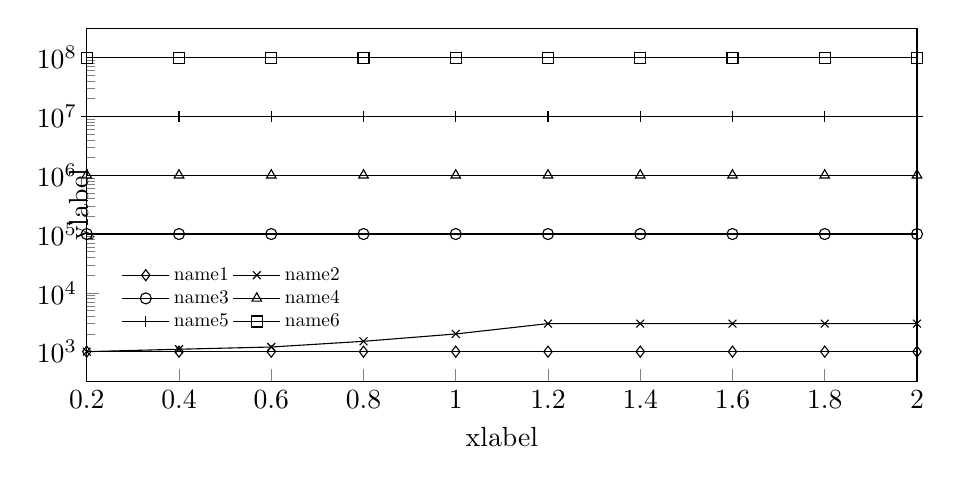
\begin{tikzpicture}
    \pgfplotstableread{
        X   name1   name2   name3   name4   name5   name6
        0.2 1e3 1e3 1e5 1e6 1e7 1e8
        0.4 1e3 1.1e3 1e5 1e6 1e7 1e8
        0.6 1e3 1.2e3 1e5 1e6 1e7 1e8
        0.8 1e3 1.5e3 1e5 1e6 1e7 1e8
        1.0 1e3 2e3 1e5 1e6 1e7 1e8
        1.2 1e3 3e3 1e5 1e6 1e7 1e8
        1.4 1e3 3e3 1e5 1e6 1e7 1e8
        1.6 1e3 3e3 1e5 1e6 1e7 1e8
        1.8 1e3 3e3 1e5 1e6 1e7 1e8
        2.0 1e3 3e3 1e5 1e6 1e7 1e8
    }{\datatable}

    \begin{axis}[
        xlabel={xlabel},
        ylabel={ylabel},
        ylabel style={at={(axis description cs:0.02,0.5)}},
        xmin= 0.2, xmax= 2.0, 
        legend style = {
            at={(0.32,0.35)},
            legend columns = {2},
            nodes={scale=0.7}, % make the legend box smaller
            fill=none,
            draw=none,
        },
        width = \linewidth,
        height = 0.5\linewidth,
        mark options={solid},
        ymode=log, % the log scale
        ytick={1e3,1e4,1e5,1e6,1e7,1e8},
        ytick pos=left, % remove the tick from the right and top
        xtick pos=bottom,
    ]
    \newcommand{\mysubplot}[2]{
        \addplot [#2] table [x=X,y=#1] {\datatable};
        \addlegendentry{#1};
    }
    \mysubplot{name1}{mark=diamond}
    \mysubplot{name2}{mark=x}
    \mysubplot{name3}{mark=o}
    \mysubplot{name4}{mark=triangle}
    \mysubplot{name5}{mark=+}
    \mysubplot{name6}{mark=square}

    \end{axis}
    \end{tikzpicture}
\end{document}